%%%%%%%%%%%%%%%%%%%%%%%%%%%%%%%%%%%%%%%%%%%%%%%%%%%%%%%%%%%%%%%%%%%%%%
% LaTeX Example: Project Report
%
% Source: http://www.howtotex.com
%
% Feel free to distribute this example, but please keep the referral
% to howtotex.com
% Date: March 2011 
% 
%%%%%%%%%%%%%%%%%%%%%%%%%%%%%%%%%%%%%%%%%%%%%%%%%%%%%%%%%%%%%%%%%%%%%%
% How to use writeLaTeX: 
%
% You edit the source code here on the left, and the preview on the
% right shows you the result within a few seconds.
%
% Bookmark this page and share the URL with your co-authors. They can
% edit at the same time!
%
% You can upload figures, bibliographies, custom classes and
% styles using the files menu.
%
% If you're new to LaTeX, the wikibook is a great place to start:
% http://en.wikibooks.org/wiki/LaTeX
%
%%%%%%%%%%%%%%%%%%%%%%%%%%%%%%%%%%%%%%%%%%%%%%%%%%%%%%%%%%%%%%%%%%%%%%
% Edit the title below to update the display in My Documents
%\title{Project Report}
%
%%% Preamble
\documentclass[paper=a4, fontsize=11pt]{scrartcl}
\usepackage[T1]{fontenc}
\usepackage{fourier}

\usepackage[english]{babel}															% English language/hyphenation
\usepackage[protrusion=true,expansion=true]{microtype}	
\usepackage{amsmath,amsfonts,amsthm} % Math packages
\usepackage[pdftex]{graphicx}	
\usepackage{url}
\usepackage{titlesec}
\usepackage{listings}
\usepackage{graphicx}


%%% Custom headers/footers (fancyhdr package)
\usepackage{fancyhdr}
\pagestyle{fancyplain}
\fancyhead{}											% No page header
\fancyfoot[L]{}											% Empty 
\fancyfoot[C]{}											% Empty
\fancyfoot[R]{\thepage}									% Pagenumbering
\renewcommand{\headrulewidth}{0pt}			% Remove header underlines
\renewcommand{\footrulewidth}{0pt}				% Remove footer underlines
\setlength{\headheight}{13.6pt}
\usepackage[margin=0.5in]{geometry}

%%% Equation and float numbering
\numberwithin{equation}{section}		% Equationnumbering: section.eq#
\numberwithin{figure}{section}			% Figurenumbering: section.fig#
\numberwithin{table}{section}				% Tablenumbering: section.tab#

%% Section Format
\titleformat*{\section}{\LARGE\bfseries}
\titleformat*{\subsection}{\Large\bfseries}
\titleformat*{\subsubsection}{\large\bfseries}
\titleformat*{\paragraph}{\large\bfseries}
\titleformat*{\subparagraph}{\large\bfseries}


%%% Maketitle metadata
\newcommand{\horrule}[1]{\rule{\linewidth}{#1}} 	% Horizontal rule

\title{
		%\vspace{-1in} 	
		\usefont{OT1}{bch}{b}{n}
		\normalfont \normalsize \textsc{University of Purdue\\
      Data Communication and Computer Networks\\
      CS 53600 Fall 2019} \\ [25pt]
		\horrule{0.5pt} \\[0.4cm]
		\huge Assignment 3\\
		\horrule{2pt} \\[0.5cm]
}
\author{
		\normalfont\normalsize Pedro da Costa Abreu Júnior\\ [-5pt]
    \normalsize Student ID 0030878383\\[-5pt]
    \normalsize \today
}
\date{}


%%% Begin document
\begin{document}
\maketitle

\section{Exercise 1 Discussions}
\subsection{}
For this exercise we run the server on pod2-2 and the client on
escher03.

We set the frame size of the server to 1472. For a completion
time of 3 seconds we need a file size of approximately 34mb.

For such we create a file with one character per line,
and for debuging purposes we set each character to a number between
0 and 9. Since each character is one byte and each line break
is also one byte we need exactly $34.000.000 / 2 = 17$ thousand lines.

For that we use the following bash script:

\begin{verbatim}
for i in {1..17000000}; do echo $(($i % 10)) >> /tmp/myfile; done
\end{verbatim}

Now we pick a port and run the server on it:

\begin{verbatim}
./myfetchfiled 1472 33449
\end{verbatim}

And we run the client three times:

\begin{verbatim}
escher03 81 $ ./myfetchfile myfile 128.10.25.207 33449
receiver: sent 6 bytes to '128.10.25.207:33449'
receiver: begining to receive file
receiver: setting up file at /tmp/myfile
receiver: file successfuly written to /tmp/myfile
receiver: completion time: 3015.006104ms
receiver: file size: 35328000 bytes
receiver: bps: 11717389.214836
receiver: Shutting Down
receiver: Good Night!

escher03 82 $ ./myfetchfile myfile 128.10.25.207 33449
receiver: sent 6 bytes to '128.10.25.207:33449'
receiver: begining to receive file
receiver: setting up file at /tmp/myfile
receiver: file successfuly written to /tmp/myfile
receiver: completion time: 3013.320068ms
receiver: file size: 35328000 bytes
receiver: bps: 11723945.415209
receiver: Shutting Down
receiver: Good Night!
escher03 83 $ ./myfetchfile myfile 128.10.25.207 33449

receiver: sent 6 bytes to '128.10.25.207:33449'
receiver: begining to receive file
receiver: setting up file at /tmp/myfile
receiver: file successfuly written to /tmp/myfile
receiver: completion time: 3014.804932ms
receiver: file size: 35328000 bytes
receiver: bps: 11718171.092673
receiver: Shutting Down
receiver: Good Night!
\end{verbatim}

We check that the received files respect the number ordering
and has the right amount of lines. This sugests that the transfer
was done correctly.

\subsection{}
To run multiple programs in parallel we do a script forking
many executions.

For two concurrent executions we get:
\begin{verbatim}
escher03 87 $ for i in {1..2}; do ./myfetchfile myfile 128.10.25.207 33449 & done
[1] 5086
[2] 5087
escher03 88 $ receiver: sent 6 bytes to '128.10.25.207:33449'
receiver: sent 6 bytes to '128.10.25.207:33449'
receiver: begining to receive file
receiver: begining to receive file
receiver: setting up file at /tmp/myfile
receiver: setting up file at /tmp/myfile
receiver: file successfuly written to /tmp/myfile
receiver: completion time: 5567.843994ms
receiver: file size: 35328000 bytes
receiver: bps: 6345005.362431
receiver: Shutting Down
receiver: Good Night!
receiver: file successfuly written to /tmp/myfile
receiver: completion time: 6036.148926ms
receiver: file size: 35328000 bytes
receiver: bps: 5852738.299598
receiver: Shutting Down
receiver: Good Night!
\end{verbatim}

As expected the completion time has doubled for each thread.

For 6 threads:
\begin{verbatim}
escher03 88 $ for i in {1..6}; do ./myfetchfile myfile 128.10.25.207 33449 & done
[1] 5294
[2] 5295
[3] 5296
[4] 5297
[5] 5298
[6] 5299
escher03 89 $ receiver: sent 6 bytes to '128.10.25.207:33449'
receiver: sent 6 bytes to '128.10.25.207:33449'
receiver: sent 6 bytes to '128.10.25.207:33449'
receiver: sent 6 bytes to '128.10.25.207:33449'
receiver: sent 6 bytes to '128.10.25.207:33449'
receiver: sent 6 bytes to '128.10.25.207:33449'
receiver: begining to receive file
receiver: begining to receive file
receiver: begining to receive file
receiver: begining to receive file
receiver: begining to receive file
receiver: begining to receive file
receiver: setting up file at /tmp/myfile
receiver: setting up file at /tmp/myfile
receiver: setting up file at /tmp/myfile
receiver: setting up file at /tmp/myfile
receiver: setting up file at /tmp/myfile
receiver: setting up file at /tmp/myfile
receiver: file successfuly written to /tmp/myfile
receiver: completion time: 16159.125977ms
receiver: file size: 35328000 bytes
receiver: bps: 2186256.858894
receiver: Shutting Down
receiver: Good Night!
receiver: file successfuly written to /tmp/myfile
receiver: completion time: 16161.904053ms
receiver: file size: 35328000 bytes
receiver: bps: 2185881.062326
receiver: Shutting Down
receiver: Good Night!
receiver: file successfuly written to /tmp/myfile
receiver: completion time: 17398.770020ms
receiver: file size: 35328000 bytes
receiver: bps: 2030488.359829
receiver: Shutting Down
receiver: Good Night!
receiver: file successfuly written to /tmp/myfile
receiver: completion time: 18018.843018ms
receiver: file size: 35328000 bytes
receiver: bps: 1960614.228424
receiver: Shutting Down
receiver: Good Night!
receiver: file successfuly written to /tmp/myfile
receiver: completion time: 18048.092041ms
receiver: file size: 35328000 bytes
receiver: bps: 1957436.825993
receiver: Shutting Down
receiver: Good Night!
receiver: file successfuly written to /tmp/myfile
receiver: completion time: 18104.608887ms
receiver: file size: 35328000 bytes
receiver: bps: 1951326.329171
receiver: Shutting Down
receiver: Good Night!
\end{verbatim}

As expected the execution time has increased by a factor of roughly 6 for each thread.

For 10 threads:
\begin{verbatim}
escher03 90 $ receiver: sent 6 bytes to '128.10.25.207:33449'
receiver: sent 6 bytes to '128.10.25.207:33449'
receiver: sent 6 bytes to '128.10.25.207:33449'
receiver: sent 6 bytes to '128.10.25.207:33449'
receiver: sent 6 bytes to '128.10.25.207:33449'
receiver: sent 6 bytes to '128.10.25.207:33449'
receiver: begining to receive file
receiver: begining to receive file
receiver: begining to receive file
receiver: sent 6 bytes to '128.10.25.207:33449'
receiver: begining to receive file
receiver: begining to receive file
receiver: sent 6 bytes to '128.10.25.207:33449'
receiver: begining to receive file
receiver: sent 6 bytes to '128.10.25.207:33449'
receiver: sent 6 bytes to '128.10.25.207:33449'
receiver: begining to receive file
receiver: begining to receive file
receiver: setting up file at /tmp/myfile
receiver: setting up file at /tmp/myfile
receiver: setting up file at /tmp/myfile
receiver: setting up file at /tmp/myfile
receiver: setting up file at /tmp/myfile
receiver: setting up file at /tmp/myfile
receiver: setting up file at /tmp/myfile
receiver: setting up file at /tmp/myfile
receiver: begining to receive file
receiver: begining to receive file
receiver: setting up file at /tmp/myfile
receiver: setting up file at /tmp/myfile
receiver: file successfuly written to /tmp/myfile
receiver: completion time: 23779.582031ms
receiver: file size: 35328000 bytes
receiver: bps: 1485644.278927
receiver: Shutting Down
receiver: Good Night!
receiver: file successfuly written to /tmp/myfile
receiver: completion time: 27433.058838ms
receiver: file size: 35328000 bytes
receiver: bps: 1287789.313206
receiver: Shutting Down
receiver: Good Night!
receiver: file successfuly written to /tmp/myfile
receiver: completion time: 27689.303955ms
receiver: file size: 35328000 bytes
receiver: bps: 1275871.724956
receiver: Shutting Down
receiver: Good Night!
receiver: file successfuly written to /tmp/myfile
receiver: completion time: 28481.589111ms
receiver: file size: 35328000 bytes
receiver: bps: 1240380.228151
receiver: Shutting Down
receiver: Good Night!
receiver: file successfuly written to /tmp/myfile
receiver: completion time: 29242.376953ms
receiver: file size: 35328000 bytes
receiver: bps: 1208109.725712
receiver: Shutting Down
receiver: Good Night!
receiver: file successfuly written to /tmp/myfile
receiver: completion time: 29592.072998ms
receiver: file size: 35328000 bytes
receiver: bps: 1193833.226970
receiver: Shutting Down
receiver: Good Night!
receiver: file successfuly written to /tmp/myfile
receiver: completion time: 29834.863037ms
receiver: file size: 35328000 bytes
receiver: bps: 1184118.055312
receiver: Shutting Down
receiver: Good Night!
receiver: file successfuly written to /tmp/myfile
receiver: completion time: 30140.389893ms
receiver: file size: 35328000 bytes
receiver: bps: 1172114.897183
receiver: Shutting Down
receiver: Good Night!
receiver: file successfuly written to /tmp/myfile
receiver: completion time: 30202.682861ms
receiver: file size: 35328000 bytes
receiver: bps: 1169697.412717
receiver: Shutting Down
receiver: Good Night!
receiver: file successfuly written to /tmp/myfile
receiver: completion time: 30208.816895ms
receiver: file size: 35328000 bytes
receiver: bps: 1169459.900510
receiver: Shutting Down
receiver: Good Night!
\end{verbatim}

As expected the completion time has increased by a factor of approximately 10.

\subsection{Varying block size}
Running every block size 10 times and taking the average on them
we get the following run times:

\begin{table}[h]
\begin{tabular}{|l|l|}
  \hline
 Block Size &  Completion Time (ms) \\
 500        &  3014.307861ms \\
 10000      &  3015.312012ms \\
 50000      &  3015.166016ms\\
 100000     &  3017.062988ms\\
 \hline
\end{tabular}
\end{table}

Since the variation on this data is so small it suggests that there is
no correlation between completion time and block size on the client side.


\section{Exercise 2 Discussions}
My first idea to solve the matching problem was the following:
if the client does not receive an ACK then we store that message
timestamp and the sequence number in a variable, and when we receive
that ACK we see if the sequence number matches. But this can
match the wrong ACK with same sequence number.

In order to solve this problem my implementation adds the timestamp
to the header of the communication, so that the ACK can send the timestamp
back, this way we guarantee that the correct ACK will be matched.

In order to implement this I created the following new structs (and they can be found in ``utils.h''):

\begin{lstlisting}
typedef struct ack {
  int seqno;
  struct timeval timestamp;
} ack_t;

typedef struct packet {
  int seqno;
  struct timeval timestamp;
  char buf[1455];
} packet_t;
\end{lstlisting}

Notice that we had to shrink the max size of the buffer due to this new
timestamp. Since timeval has the size of two longs, in the worse case scenario
it will be 128 bits or 16 bytes.
Since the buffer max size is originally 1471, 1471-16 = 1455.

In order to make this work we first implement a simple linked list
on the client side, encoding all the timestamp that have been sent.
So that when we receive an ACK, we have the correct log of when that message was
sent to the client.

There were also several new corner cases that had to be handled
that were not an issue before, for example, now the server
might actually request for a package due to a timeout.
The way my client was implemented before it always knew
when the server was going to re-send a packet, and therefore it
simplified the algorithm significantly.

When running ``under the gun'' at some point the slack becomes too thin and the server
simply drops the connection.

All the other experiments worked as expected.

\section{Exercise 3 Discussions}
Using a file size of 300 and a blocksize of 30 we analyzed the
output of \texttt{tcpdumpwrap-veth0} with \texttt{wireshark}.

Running \textit{ifconfig -a} on the receiver we get:
\begin{lstlisting}
veth0: flags=4163<UP,BROADCAST,RUNNING,MULTICAST>  mtu 1500
        inet 192.168.1.1  netmask 255.255.255.0  broadcast 192.168.1.255
        inet6 fe80::ec4d:4dff:fec2:a2be  prefixlen 64  scopeid 0x20<link>
        ether ee:4d:4d:c2:a2:be  txqueuelen 1000  (Ethernet)
        RX packets 53193  bytes 12742360 (12.7 MB)
        RX errors 0  dropped 0  overruns 0  frame 0
        TX packets 696  bytes 66976 (66.9 KB)
        TX errors 0  dropped 0 overruns 0  carrier 0  collisions 0
\end{lstlisting}

This shows that the mac address of the file receiver is \texttt{ee:4d:4d:c2:a2:be}

And running \textit{veth 'ifconfig -a'} on the sender we get:
\begin{lstlisting}
veth0: flags=4163<UP,BROADCAST,RUNNING,MULTICAST>  mtu 1500
        inet 192.168.1.2  netmask 255.255.255.0  broadcast 192.168.1.255
        inet6 fe80::2c5b:78ff:fe7c:1de4  prefixlen 64  scopeid 0x20<link>
        ether 2e:5b:78:7c:1d:e4  txqueuelen 1000  (Ethernet)
        RX packets 696  bytes 66976 (66.9 KB)
        RX errors 0  dropped 0  overruns 0  frame 0
        TX packets 53193  bytes 12742360 (12.7 MB)
        TX errors 0  dropped 0 overruns 0  carrier 0  collisions 0
\end{lstlisting}

This shows that the mac address of the file sender is \texttt{2e:5b:78:7c:1d:e4}

Here is the byte output of the first message:
\begin{lstlisting}
ee 4d 4d c2 a2 be 2e 5b 78 7c 1d e4 08 00 45 00
00 3b 50 4a 40 00 40 11 67 14 c0 a8 01 02 c0 a8
01 01 82 e9 ec 96 00 27 83 8c 00 33 33 33 33 33
33 33 33 33 33 33 33 33 33 33 33 33 33 33 33 33
33 33 33 33 33 33 33 33 33
\end{lstlisting}

From this we can see that the first 6 bytes is the file receiver mac address
as captured by \texttt{ifconfig}.
The following 6 bytes is the file sender mac address, as captured by \textit{veth 'ifconfig'}.
The following 2 bytes (08 00) is the type of the connection, in this case IPv4.
In the middle of the packet we have 20 bytes of IP header and 8 bytes of UDP header.
Then at the end of the packet we have 00 33 33 ... which is the payload of the communication.
00 is the sequence number and 0x33 is the ascii code for '3'. And we have exactly 30 '3's, as expected.

Now this is the byte output of the second message:
\begin{lstlisting}
2e 5b 78 7c 1d e4 ee 4d 4d c2 a2 be 08 00 45 00
00 1d 1f 7c 40 00 40 11 98 00 c0 a8 01 01 c0 a8
01 02 b8 85 82 e9 00 09 83 6e 00
\end{lstlisting}

Similarly we have the file sender mac address as the 6 bytes and the file receiver mac address as the following 6 bytes.
The last byte (00) is the ACK of the first message (00).


The following was the last two messages with sequence number 2,
ending the communication.

\begin{lstlisting}
ee 4d 4d c2 a2 be 2e 5b 78 7c 1d e4 08 00 45 00
00 1d 50 56 40 00 40 11 67 26 c0 a8 01 02 c0 a8
01 01 82 e9 ec 96 00 09 83 6e 02
\end{lstlisting}

\begin{lstlisting}
2e 5b 78 7c 1d e4 ee 4d 4d c2 a2 be 08 00 45 00
00 1d 1f 86 40 00 40 11 97 f6 c0 a8 01 01 c0 a8
01 02 b8 85 82 e9 00 09 83 6e 02              
\end{lstlisting}

As we can see we have exactly the same message header as before
with the difference that the last byte is 2 for the sequence number ending the communication.

Also notice that in our case padding was not applied in any of the payloads.

Bellow is listed all 10 message logs found between the sender
and the receiver

\begin{lstlisting}
00000000: d4c3 b2a1 0200 0400 0000 0000 0000 0000  ................
00000010: 0000 0400 0100 0000 0edd a45d f40a 0600  ...........]....
00000020: 4900 0000 4900 0000 ee4d 4dc2 a2be 2e5b  I...I....MM....[
00000030: 787c 1de4 0800 4500 003b 504a 4000 4011  x|....E..;PJ@.@.
00000040: 6714 c0a8 0102 c0a8 0101 82e9 ec96 0027  g..............'
00000050: 838c 0033 3333 3333 3333 3333 3333 3333  ...3333333333333
00000060: 3333 3333 3333 3333 3333 3333 3333 3333  3333333333333333
00000070: 330e dda4 5d95 0b06 002b 0000 002b 0000  3...]....+...+..
00000080: 002e 5b78 7c1d e4ee 4d4d c2a2 be08 0045  ..[x|...MM.....E
00000090: 0000 1d1f 7c40 0040 1198 00c0 a801 01c0  ....|@.@........
000000a0: a801 02b8 8582 e900 0983 6e00 0edd a45d  ..........n....]
000000b0: df0b 0600 4900 0000 4900 0000 ee4d 4dc2  ....I...I....MM.
000000c0: a2be 2e5b 787c 1de4 0800 4500 003b 504b  ...[x|....E..;PK
000000d0: 4000 4011 6713 c0a8 0102 c0a8 0101 82e9  @.@.g...........
000000e0: ec96 0027 838c 0133 3333 3333 3333 3333  ...'...333333333
000000f0: 3333 3333 3333 3333 3333 3333 3333 3333  3333333333333333
00000100: 3333 3333 330e dda4 5d52 0c06 002b 0000  33333...]R...+..
00000110: 002b 0000 002e 5b78 7c1d e4ee 4d4d c2a2  .+....[x|...MM..
00000120: be08 0045 0000 1d1f 7d40 0040 1197 ffc0  ...E....}@.@....
00000130: a801 01c0 a801 02b8 8582 e900 0983 6e01  ..............n.
00000140: 0edd a45d af0c 0600 4900 0000 4900 0000  ...]....I...I...
00000150: ee4d 4dc2 a2be 2e5b 787c 1de4 0800 4500  .MM....[x|....E.
00000160: 003b 504c 4000 4011 6712 c0a8 0102 c0a8  .;PL@.@.g.......
00000170: 0101 82e9 ec96 0027 838c 0033 3333 3333  .......'...33333
00000180: 3333 3333 3333 3333 3333 3333 3333 3333  3333333333333333
00000190: 3333 3333 3333 3333 330e dda4 5d28 0d06  333333333...](..
000001a0: 002b 0000 002b 0000 002e 5b78 7c1d e4ee  .+...+....[x|...
000001b0: 4d4d c2a2 be08 0045 0000 1d1f 7e40 0040  MM.....E....~@.@
000001c0: 1197 fec0 a801 01c0 a801 02b8 8582 e900  ................
000001d0: 0983 6e00 0edd a45d 700d 0600 4900 0000  ..n....]p...I...
000001e0: 4900 0000 ee4d 4dc2 a2be 2e5b 787c 1de4  I....MM....[x|..
000001f0: 0800 4500 003b 504d 4000 4011 6711 c0a8  ..E..;PM@.@.g...
00000200: 0102 c0a8 0101 82e9 ec96 0027 838c 0133  ...........'...3
00000210: 3333 3333 3333 3333 3333 3333 3333 3333  3333333333333333
00000220: 3333 3333 3333 3333 3333 3333 330e dda4  3333333333333...
00000230: 5de2 0d06 002b 0000 002b 0000 002e 5b78  ]....+...+....[x
00000240: 7c1d e4ee 4d4d c2a2 be08 0045 0000 1d1f  |...MM.....E....
00000250: 7f40 0040 1197 fdc0 a801 01c0 a801 02b8  .@.@............
00000260: 8582 e900 0983 6e01 0edd a45d 2f0e 0600  ......n....]/...
00000270: 4900 0000 4900 0000 ee4d 4dc2 a2be 2e5b  I...I....MM....[
00000280: 787c 1de4 0800 4500 003b 504e 4000 4011  x|....E..;PN@.@.
00000290: 6710 c0a8 0102 c0a8 0101 82e9 ec96 0027  g..............'
000002a0: 838c 0033 3333 3333 3333 3333 3333 3333  ...3333333333333
000002b0: 3333 3333 3333 3333 3333 3333 3333 3333  3333333333333333
000002c0: 330e dda4 5d05 1606 0049 0000 0049 0000  3...]....I...I..
000002d0: 00ee 4d4d c2a2 be2e 5b78 7c1d e408 0045  ..MM....[x|....E
000002e0: 0000 3b50 4f40 0040 1167 0fc0 a801 02c0  ..;PO@.@.g......
000002f0: a801 0182 e9ec 9600 2783 8c00 3333 3333  ........'...3333
00000300: 3333 3333 3333 3333 3333 3333 3333 3333  3333333333333333
00000310: 3333 3333 3333 3333 3333 0edd a45d 7616  3333333333...]v.
00000320: 0600 2b00 0000 2b00 0000 2e5b 787c 1de4  ..+...+....[x|..
00000330: ee4d 4dc2 a2be 0800 4500 001d 1f80 4000  .MM.....E.....@.
00000340: 4011 97fc c0a8 0101 c0a8 0102 b885 82e9  @...............
00000350: 0009 836e 000e dda4 5db0 1606 0049 0000  ...n....]....I..
00000360: 0049 0000 00ee 4d4d c2a2 be2e 5b78 7c1d  .I....MM....[x|.
00000370: e408 0045 0000 3b50 5040 0040 1167 0ec0  ...E..;PP@.@.g..
00000380: a801 02c0 a801 0182 e9ec 9600 2783 8c01  ............'...
00000390: 3333 3333 3333 3333 3333 3333 3333 3333  3333333333333333
000003a0: 3333 3333 3333 3333 3333 3333 3333 0edd  33333333333333..
000003b0: a45d 1f17 0600 2b00 0000 2b00 0000 2e5b  .]....+...+....[
000003c0: 787c 1de4 ee4d 4dc2 a2be 0800 4500 001d  x|...MM.....E...
000003d0: 1f81 4000 4011 97fb c0a8 0101 c0a8 0102  ..@.@...........
000003e0: b885 82e9 0009 836e 010e dda4 5d7c 1706  .......n....]|..
000003f0: 0049 0000 0049 0000 00ee 4d4d c2a2 be2e  .I...I....MM....
00000400: 5b78 7c1d e408 0045 0000 3b50 5140 0040  [x|....E..;PQ@.@
00000410: 1167 0dc0 a801 02c0 a801 0182 e9ec 9600  .g..............
00000420: 2783 8c00 3333 3333 3333 3333 3333 3333  '...333333333333
00000430: 3333 3333 3333 3333 3333 3333 3333 3333  3333333333333333
00000440: 3333 0edd a45d f017 0600 2b00 0000 2b00  33...]....+...+.
00000450: 0000 2e5b 787c 1de4 ee4d 4dc2 a2be 0800  ...[x|...MM.....
00000460: 4500 001d 1f82 4000 4011 97fa c0a8 0101  E.....@.@.......
00000470: c0a8 0102 b885 82e9 0009 836e 000e dda4  ...........n....
00000480: 5d2d 1806 0049 0000 0049 0000 00ee 4d4d  ]-...I...I....MM
00000490: c2a2 be2e 5b78 7c1d e408 0045 0000 3b50  ....[x|....E..;P
000004a0: 5240 0040 1167 0cc0 a801 02c0 a801 0182  R@.@.g..........
000004b0: e9ec 9600 2783 8c01 3333 3333 3333 3333  ....'...33333333
000004c0: 3333 3333 3333 3333 3333 3333 3333 3333  3333333333333333
000004d0: 3333 3333 3333 0edd a45d 5d18 0600 2b00  333333...]]...+.
000004e0: 0000 2b00 0000 2e5b 787c 1de4 ee4d 4dc2  ..+....[x|...MM.
000004f0: a2be 0800 4500 001d 1f83 4000 4011 97f9  ....E.....@.@...
00000500: c0a8 0101 c0a8 0102 b885 82e9 0009 836e  ...............n
00000510: 010e dda4 5d8a 1806 0049 0000 0049 0000  ....]....I...I..
00000520: 00ee 4d4d c2a2 be2e 5b78 7c1d e408 0045  ..MM....[x|....E
00000530: 0000 3b50 5340 0040 1167 0bc0 a801 02c0  ..;PS@.@.g......
00000540: a801 0182 e9ec 9600 2783 8c00 3333 3333  ........'...3333
00000550: 3333 3333 3333 3333 3333 3333 3333 3333  3333333333333333
00000560: 3333 3333 3333 3333 3333 0edd a45d 7620  3333333333...]v
00000570: 0600 4900 0000 4900 0000 ee4d 4dc2 a2be  ..I...I....MM...
00000580: 2e5b 787c 1de4 0800 4500 003b 5054 4000  .[x|....E..;PT@.
00000590: 4011 670a c0a8 0102 c0a8 0101 82e9 ec96  @.g.............
000005a0: 0027 838c 0033 3333 3333 3333 3333 3333  .'...33333333333
000005b0: 3333 3333 3333 3333 3333 3333 3333 3333  3333333333333333
000005c0: 3333 330e dda4 5dac 2006 002b 0000 002b  333...]. ..+...+
000005d0: 0000 002e 5b78 7c1d e4ee 4d4d c2a2 be08  ....[x|...MM....
000005e0: 0045 0000 1d1f 8440 0040 1197 f8c0 a801  .E.....@.@......
000005f0: 01c0 a801 02b8 8582 e900 0983 6e00 0edd  ............n...
00000600: a45d e220 0600 4900 0000 4900 0000 ee4d  .]. ..I...I....M
00000610: 4dc2 a2be 2e5b 787c 1de4 0800 4500 003b  M....[x|....E..;
00000620: 5055 4000 4011 6709 c0a8 0102 c0a8 0101  PU@.@.g.........
00000630: 82e9 ec96 0027 838c 0133 3333 3333 3333  .....'...3333333
00000640: 3333 3333 3333 3333 3333 3333 3333 3333  3333333333333333
00000650: 3333 3333 3333 330e dda4 5d0d 2106 002b  3333333...].!..+
00000660: 0000 002b 0000 002e 5b78 7c1d e4ee 4d4d  ...+....[x|...MM
00000670: c2a2 be08 0045 0000 1d1f 8540 0040 1197  .....E.....@.@..
00000680: f7c0 a801 01c0 a801 02b8 8582 e900 0983  ................
00000690: 6e01 0edd a45d 4221 0600 2b00 0000 2b00  n....]B!..+...+.
000006a0: 0000 ee4d 4dc2 a2be 2e5b 787c 1de4 0800  ...MM....[x|....
000006b0: 4500 001d 5056 4000 4011 6726 c0a8 0102  E...PV@.@.g&....
000006c0: c0a8 0101 82e9 ec96 0009 836e 020e dda4  ...........n....
000006d0: 5d73 2106 002b 0000 002b 0000 002e 5b78  ]s!..+...+....[x
000006e0: 7c1d e4ee 4d4d c2a2 be08 0045 0000 1d1f  |...MM.....E....
000006f0: 8640 0040 1197 f6c0 a801 01c0 a801 02b8  .@.@............
00000700: 8582 e900 0983 6e02 0a                   ......n..
\end{lstlisting}


At the figure bellow we can see a picture of wireshark, great a tool
to help us analyze the traffic logs.

\begin{figure}[h]
  \centering
  \label{fig:wireshark}
  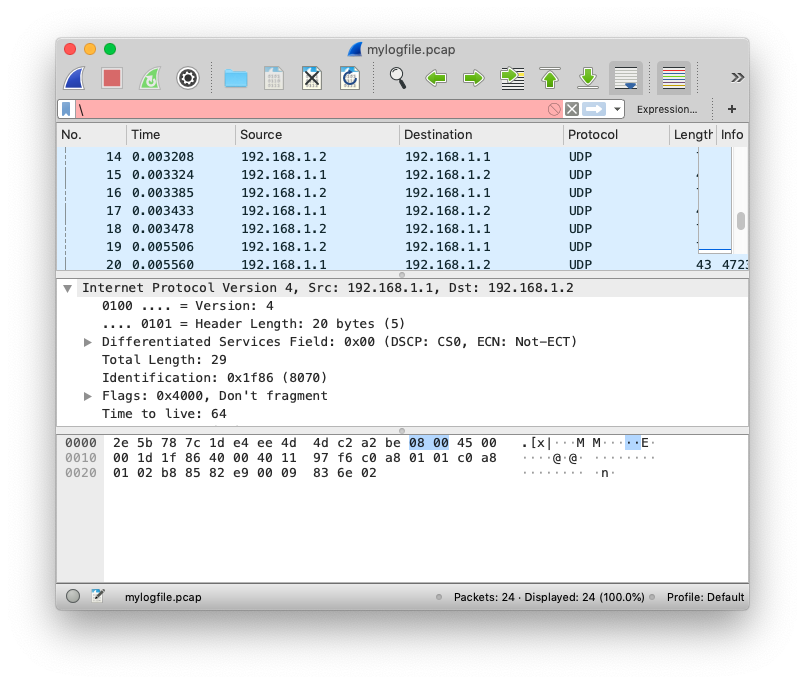
\includegraphics[width=\textwidth]{wireshark}
  \caption{Screenshot of wireshark with the communication log}
\end{figure}
%%% End document
\end{document}
